\documentclass[11pt,oneside]{report}

\usepackage[a4paper,margin=2.5cm]{geometry}
\usepackage[T1]{fontenc}
\usepackage{lmodern}
\usepackage[english]{babel}
\usepackage{microtype}
\usepackage{graphicx}
\graphicspath{{reports/assets/}{assets/}}
\usepackage{booktabs}
\usepackage{tabularx}
\usepackage{longtable}
\usepackage{array}
\usepackage{ragged2e}
\usepackage{amsmath}
\usepackage{amssymb}
\usepackage{mathtools}
\usepackage{tikz}
\usetikzlibrary{arrows.meta,positioning,fit}
\usepackage{caption}
\usepackage{xurl}
\usepackage[hidelinks]{hyperref}

\hypersetup{
  pdftitle={NYC Crime Intelligence: Model, Training, and Dashboard},
  pdfsubject={Technical project report},
  pdfauthor={Mert Samet Kayacıoğlu}
}

\pagestyle{plain}
\renewcommand{\arraystretch}{1.15}
\setcounter{tocdepth}{2}

\newcolumntype{Y}{>{\RaggedRight\arraybackslash}X}
\newcolumntype{R}{>{\RaggedLeft\arraybackslash}X}

\newenvironment{summarybox}[1][]
  {\begin{quote}\small\noindent\textbf{#1}\par\smallskip}
  {\end{quote}}

\newenvironment{warningbox}[1][]
  {\begin{quote}\small\noindent\textbf{#1}\par\smallskip}
  {\end{quote}}

\newcommand{\metric}[2]{%
  \begin{minipage}[t]{0.23\textwidth}
    \centering
    {\bfseries\large #1}\par
    {\small #2}
  \end{minipage}%
}

\title{NYC Crime Intelligence\\[0.75em]
  \large Model, Training, and Dashboard}
\author{Mert Samet Kayacıoğlu\\[0.5em]
  \small Technical Project Report\\
  \small Aggregate analytics only}
\date{July 19, 2026}

\begin{document}
\pagenumbering{gobble}
\maketitle

\pagenumbering{roman}

\chapter*{Executive Summary}
\addcontentsline{toc}{chapter}{Executive Summary}

NYC Crime Intelligence is an aggregate-only analytical system built from the
official NYPD Complaint Data Historic dataset. The project converts a reviewed
10,071,507-row source snapshot into deterministic weekly aggregates, evaluates
transparent forecasting rules, produces retrospective hotspot and anomaly
signals, and presents the results in a local React dashboard. The system is
designed for exploratory analysis of reported complaint patterns, not for
person-level prediction or operational policing decisions \cite{finalreport,rootreadme}.

\begin{center}
  \metric{10.07M}{source rows}\hfill
  \metric{8,466}{aggregate segments}\hfill
  \metric{0.4894}{ML backtest MAE}\hfill
  \metric{6}{dashboard experiences}
\end{center}

\begin{summarybox}[Core result]
The selected \texttt{duckdb\_lag\_ensemble\_regressor} slightly outperforms the
best deterministic baseline on the recorded time-based backtest: MAE decreases
from 0.4929 to 0.4894 and RMSE from 1.4128 to 1.3943. The improvement is small,
the two summaries have different prediction coverage, and the model emits point
estimates without prediction intervals. The dashboard therefore presents model
outputs together with historical error context and explicit limitations.
\end{summarybox}

The report is organized in two parts. Part I documents the data foundation,
model design, training logic, leakage controls, backtest results, and governance
constraints. Part II explains the dashboard architecture, analytical views,
filter behavior, accessibility design, deployment workflow, and verification
strategy.

\tableofcontents
\clearpage

\pagenumbering{arabic}

\part{Model Development and Training}

\chapter{Problem Definition and Data Foundation}

\section{Analytical objective}

The forecasting task is to estimate the next week's reported complaint count
for each aggregate segment:

\begin{equation}
  \text{week\_start} \times \text{borough} \times \text{precinct}
  \times \text{offense\_type} \times \text{law\_category}.
\end{equation}

The target is a count of date-eligible source rows, not a count of unique
incidents, people, victims, harms, or causal effects. The forecast unit is an
area/category segment. Exact addresses, exact event coordinates, complaint
identifiers, names, and victim or suspect demographic fields are outside the
modeling scope \cite{cleaningreport,finalreport}.

The project addresses three aggregate questions:

\begin{enumerate}
  \item How does reported complaint volume vary over time and across geography
    and offense categories?
  \item Which already-observed aggregates show unusual concentration or a high
    deviation from prior-only history?
  \item For one fixed week, how does an explainable lag-based estimate compare
    with a transparent historical baseline?
\end{enumerate}

\section{Source snapshot and eligibility rule}

The analytical source is NYC Open Data's \emph{NYPD Complaint Data Historic}
dataset, identifier \nolinkurl{qgea-i56i}. The reviewed local CSV is 3.19 GB and
has SHA-256 checksum
\nolinkurl{759016def1c04aafaaeaa8e35c622d13abdd4af82a69f7b9e2b5549c08e47827}.
The exact source bytes are excluded from Git; a newer portal export constitutes
a different analytical snapshot \cite{provenance}.

The deterministic cleaning stage reads reviewed columns as text, normalizes
null-like tokens, trims and standardizes categorical values, parses dates with
\texttt{\%m/\%d/\%Y}, and uses safe numeric casts. A row enters the aggregate
dataset only if its canonical complaint start date:

\begin{itemize}
  \item parses successfully;
  \item is on or after January 1, 2006; and
  \item is on or before the explicit review date, July 4, 2026.
\end{itemize}

Other data-quality conditions are retained as audit flags. Missing dimensions
do not by themselves remove a date-eligible row: missing borough, precinct, or
offense values are represented by the literal category \texttt{UNKNOWN}.

\begin{table}[htbp]
  \centering
  \caption{Reviewed source and aggregate populations.}
  \label{tab:data-populations}
  \begin{tabularx}{0.83\textwidth}{Y r}
    \toprule
    Population & \textbf{Rows} \\
    \midrule
    Source rows evaluated & 10,071,507 \\
    Rows included in aggregates & 10,049,687 \\
    Rows excluded by date eligibility & 21,820 \\
    Weekly aggregate rows & 1,761,447 \\
    Distinct aggregate segments used by forecasting & 8,466 \\
    \bottomrule
  \end{tabularx}
\end{table}

Quality flags can overlap: 52,050 rows have at least one listed flag and 605
have more than one. Consequently, individual flag counts must not be summed or
equated with the 21,820 date-based exclusions \cite{qualityreport}.

\section{Weekly panel construction}

DuckDB's \texttt{date\_trunc('week', ...)} creates Monday-starting buckets. The
eligible event dates run from January 1, 2006 through December 31, 2025, while
bucket labels run from December 26, 2005 through December 29, 2025. The first
label is earlier than event coverage because January 1, 2006 is a Sunday in the
week beginning December 26, 2005.

Missing segment-weeks are filled with zero only after the segment first appears.
This rule creates a complete post-appearance panel without inventing an earlier
history. It is useful for lag calculations but cannot distinguish a true zero
from an upstream reporting absence.

The final bucket, beginning December 29, 2025, contains only Monday through
Wednesday. It is excluded from baseline backtesting and anomaly scoring, yet it
is retained as the latest observation for the fixed forecast. This asymmetry is
intentional, but it can depress lag-based inputs relative to a complete seven-day
week.

\begin{figure}[htbp]
  \centering
  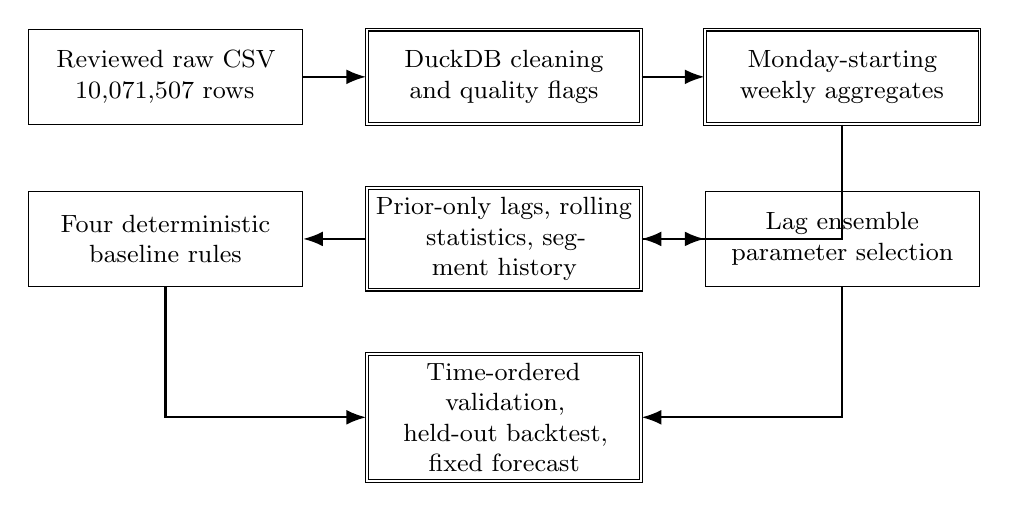
\begin{tikzpicture}[
    node distance=8mm and 8mm,
    block/.style={draw=black,
      minimum height=12mm, text width=3.25cm, align=center,
      font=\small},
    active/.style={block, double},
    arrow/.style={-{Latex[length=2.5mm]}, thick}
  ]
    \node[block] (raw) {Reviewed raw CSV\\10,071,507 rows};
    \node[active, right=of raw] (clean) {DuckDB cleaning\\and quality flags};
    \node[active, right=of clean] (weekly) {Monday-starting\\weekly aggregates};
    \node[active, below=of clean] (features) {Prior-only lags, rolling\\statistics, segment history};
    \node[block, left=of features] (baseline) {Four deterministic\\baseline rules};
    \node[block, right=of features] (model) {Lag ensemble\\parameter selection};
    \node[active, below=of features] (evaluate) {Time-ordered validation,\\held-out backtest, fixed forecast};
    \draw[arrow] (raw) -- (clean);
    \draw[arrow] (clean) -- (weekly);
    \draw[arrow] (weekly) |- (features);
    \draw[arrow] (features) -- (baseline);
    \draw[arrow] (features) -- (model);
    \draw[arrow] (baseline) |- (evaluate);
    \draw[arrow] (model) |- (evaluate);
  \end{tikzpicture}
  \caption{Model development pipeline. Every model input is derived from
  aggregate history and uses prior weeks only.}
  \label{fig:model-pipeline}
\end{figure}

\chapter{Baseline and Lag-Ensemble Model}

\section{Deterministic baselines}

Four target-week-excluding baseline rules are evaluated for each segment. If
$y_{s,t}$ is the count for segment $s$ in week $t$, the rules are:

\begin{align}
  \widehat{y}^{(1)}_{s,t} &= y_{s,t-1}, \\
  \widehat{y}^{(4)}_{s,t} &= \frac{1}{4}\sum_{i=1}^{4} y_{s,t-i}, \\
  \widehat{y}^{(8)}_{s,t} &= \frac{1}{8}\sum_{i=1}^{8} y_{s,t-i}, \\
  \widehat{y}^{(52)}_{s,t} &= y_{s,t-52}.
\end{align}

The trailing eight-week arithmetic mean is selected by overall MAE. It covers
99.73\% of the recorded backtest and provides a strong, interpretable reference
for the lag ensemble \cite{baselinereport,baselinemanifest}.

\begin{table}[htbp]
  \centering
  \caption{Baseline performance on the December 30, 2024--December 22, 2025
  backtest window. Lower errors are better.}
  \label{tab:baseline-results}
  \begin{tabular}{lrrrr}
    \toprule
    \textbf{Method} & \textbf{Coverage} & \textbf{MAE} & \textbf{RMSE} & \textbf{Weighted MAE} \\
    \midrule
    Previous week & 99.97\% & 0.6010 & 1.7764 & 4.5649 \\
    Previous year, same week & 97.64\% & 0.6796 & 2.0772 & 5.2965 \\
    Trailing four-week mean & 99.87\% & 0.5058 & 1.4537 & 3.7967 \\
    \textbf{Trailing eight-week mean} & \textbf{99.73\%} & \textbf{0.4929} & \textbf{1.4128} & \textbf{3.7023} \\
    \bottomrule
  \end{tabular}
\end{table}

\section{Feature engineering}

The model manifest records a broad, auditable feature context:

\begin{itemize}
  \item calendar variables: year, month, ISO week, quarter, and sequential week
    index;
  \item count lags at 1, 2, 4, 8, and 52 weeks;
  \item trailing four- and eight-week mean, standard deviation, minimum, and
    maximum;
  \item prior segment count, cumulative total, and mean; and
  \item borough, precinct, offense type, and law category identifiers.
\end{itemize}

Only four numeric inputs enter the deployed prediction formula: the one-week
lag, the 52-week lag, and the trailing four- and eight-week means. The remaining
engineered fields are retained as audit context rather than silently presented
as formula inputs. Missing lag or rolling inputs fall back to available prior
segment history and then to zero \cite{mlmanifest}.

\section{Model identity and prediction rule}

The reviewed estimator is \texttt{duckdb\_lag\_ensemble\_regressor}, model
version 1 and artifact version 1. It is a deterministic formula implemented
with the Python standard library and DuckDB; it does not persist a binary
scikit-learn estimator. This choice makes the release portable and permits a
direct audit of every prediction.

Let $m_{4,s,t}$ and $m_{8,s,t}$ denote prior-only four- and eight-week means,
and let $\ell_{1,s,t}$ and $\ell_{52,s,t}$ denote one- and 52-week lags. The
forecast is:

\begin{equation}
\widehat{y}_{s,t} = \max\left\{0,\,\lambda\left[
 m_{8,s,t}
 + \alpha(m_{4,s,t}-m_{8,s,t})
 + \beta(\ell_{1,s,t}-m_{4,s,t})
 + \gamma(\ell_{52,s,t}-m_{8,s,t})
\right]\right\}.
\label{eq:model}
\end{equation}

The selected parameters are $\alpha=0.25$, $\beta=0.10$, $\gamma=0.05$, and
$\lambda=1.0$. The terms have intuitive roles: the eight-week mean is the
anchor, the four-week term introduces recent momentum, the one-week term adds a
short-run correction, and the 52-week term contributes a modest seasonal
adjustment. The outer maximum prevents negative count estimates.

\begin{summarybox}[Why this model fits the project]
The estimator is intentionally conservative. It improves on a strong moving
average without obscuring the calculation behind a serialized black-box model.
This matches the project's emphasis on aggregate analysis, reproducibility,
auditability, and explicit responsible-use limits.
\end{summarybox}

\section{Training and evaluation chronology}

Random train/test splits are not used. Parameter selection is evaluated on a
time-ordered validation window, followed by a later held-out backtest. The
fixed forecast uses all available prior aggregate history through the partial
week beginning December 29, 2025.

\clearpage
\begin{center}
  \centering
  \captionsetup{hypcap=false}
  \captionof{table}{Model lifecycle and evaluation windows.}
  \label{tab:model-windows}
  \begin{tabularx}{\textwidth}{>{\bfseries}p{0.29\textwidth} Y}
    \toprule
    Field & Value and interpretation \\
    \midrule
    Aggregate history & December 26, 2005--December 29, 2025; the first label is a week boundary, not 2005 event coverage. \\
    Parameter validation & January 1--December 23, 2024; selection objective is validation RMSE. \\
    Held-out backtest & December 30, 2024--December 22, 2025; the final partial bucket is excluded. \\
    Fixed forecast week & January 5, 2026. \\
    Artifact generated & July 5, 2026 at 12:40:05 UTC. \\
    Training completion & Not independently recorded; artifact generation time must not be relabeled as training completion. \\
    \bottomrule
  \end{tabularx}
\end{center}

The target week precedes artifact construction. The output is therefore a
fixed retrospective demonstration rather than a rolling or real-time service.

\chapter{Evaluation, Interpretation, and Governance}

\section{Backtest results}

The lag ensemble generates predictions for all 437,144 backtest segment-weeks.
Table~\ref{tab:model-comparison} summarizes the recorded overall results.

\begin{table}[htbp]
  \centering
  \caption{Selected baseline and lag-ensemble backtest metrics.}
  \label{tab:model-comparison}
  \begin{tabular}{lrrrr}
    \toprule
    \textbf{Model} & \textbf{Coverage} & \textbf{MAE} & \textbf{RMSE} & \textbf{Weighted MAE} \\
    \midrule
    Trailing eight-week baseline & 99.73\% & 0.4929 & 1.4128 & 3.7023 \\
    Lag ensemble & 100.00\% & 0.4894 & 1.3943 & 3.6555 \\
    \midrule
    Difference: ML $-$ baseline & +0.27 pp & $-0.0035$ & $-0.0185$ & $-0.0468$ \\
    \bottomrule
  \end{tabular}
\end{table}

The ML model improves all three reported error metrics, but the improvement is
small. Moreover, the baseline and ML summaries contain different numbers of
predictions (435,942 versus 437,144), so the differences are descriptive rather
than a matched-row causal comparison. They should not be reported as guaranteed
performance gains for a selected borough, precinct, offense, or law category.

The error distribution is also heterogeneous. High-volume and volatile series,
including several petit larceny and harassment precinct/offense segments, have
substantially larger errors than the overall average \cite{mlreport}.

\section{Leakage controls and reproducibility}

The pipeline applies the following controls:

\begin{itemize}
  \item every lag and rolling statistic excludes the target week;
  \item validation precedes backtesting in calendar time;
  \item random splits are disabled;
  \item the latest partial week is excluded from the backtest;
  \item zero filling begins only after a segment's first observation; and
  \item generated artifacts use deterministic ordering and stable,
    repository-relative references.
\end{itemize}

The canonical rebuild order is the cleaning stage, dashboard summary, baseline,
ML model, hotspots, anomalies, and the browser projections. A complete
reproduction requires the raw CSV whose checksum matches the recorded source
snapshot. Changing the source checksum or the explicit review date creates a
different analytical release.

\section{Limitations}

\begin{warningbox}[Interpretation limits]
Reported complaint counts reflect reporting behavior, delay, revision,
under-reporting, classification, and policy change. They are neither complete
measures of harm nor causal truth. Model output is a point estimate and does not
include a prediction interval, calibration analysis, filter-specific error, or
formal drift monitoring.
\end{warningbox}

Important technical limitations include:

\begin{itemize}
  \item the latest input bucket contains only three days;
  \item post-appearance zero filling may confuse a genuine zero with an
    upstream reporting gap;
  \item the formula omits holidays, reporting-delay corrections, exogenous
    events, spatial spillover, and explicit structural-break terms;
  \item the reported improvement is based on one historical split;
  \item the model has no general retraining cadence or model-age service
    threshold; and
  \item browser forecast geography withholds 2,614 model rows that cannot be
    mapped safely to the reviewed precinct contract.
\end{itemize}

The browser-safe forecast subset contains 5,852 rows across 78 precincts. This
retains 69.12\% of model rows but 99.62\% of predicted volume. Expected Change
has a baseline for 5,848 rows; four rows lack sufficient history, while 3,051
valid zero baselines make percentage change mathematically undefined.

\section{Privacy and responsible use}

Sensitive suspect and victim demographic fields are excluded from the cleaned
modeling projection and all forecast features. The model does not generate an
individual risk score, a future-incident location, or a patrol, enforcement,
deployment, intervention, or resource-allocation recommendation.

Appropriate use is limited to transparent, retrospective exploration of
aggregate reported-complaint patterns and model error. Hotspot and anomaly
severity must not be interpreted as offense seriousness, neighborhood danger,
or policing priority.

\part{Dashboard Design and Implementation}

\chapter{Dashboard Architecture}

\section{Technology stack and deployment model}

The dashboard is a local single-page application implemented with React 19,
TypeScript 6, and Vite 8. Recharts renders analytical charts and Leaflet renders
spatial layers. The application has no API, scheduler, update channel, or
long-running analytical service. Instead, it loads committed, browser-safe
artifacts produced by the Python and DuckDB pipeline \cite{dashboardreadme}.

The recommended local launcher is:

\begin{verbatim}
./run.sh
\end{verbatim}

The launcher validates Node.js and npm, installs locked dependencies when
necessary, and starts Vite at \url{http://127.0.0.1:4173/}. The supported Node
range is \texttt{\string^20.19.0 || \string^22.13.0 || >=24.0.0}, with npm 10 or newer.

\section{Browser-safe data contracts}

The application loads five staged artifacts:

\begin{table}[htbp]
  \centering
  \caption{Dashboard artifacts and their primary consumers.}
  \label{tab:dashboard-artifacts}
  \begin{tabularx}{\textwidth}{>{\small\RaggedRight\arraybackslash}p{0.46\textwidth} Y}
    \toprule
    \normalfont\bfseries Artifact & \bfseries Role \\
    \midrule
    \path{public/data/overview.json} & Metadata, governance fields, filters, summaries, and anomaly projection. \\
    \path{public/data/overview-cube.bin.gz} & Compressed weekly cube used for observed totals and charts. \\
    \path{public/data/map.json} & Fixed retrospective hotspot snapshot and list/detail data. \\
    \path{public/data/forecast-map.json} & Precinct-level fixed forecast and Expected Change values. \\
    \path{public/data/precinct-spatial-reference.json} & Reviewed 78-feature official precinct geometry. \\
    \bottomrule
  \end{tabularx}
\end{table}

Every loader treats incoming JSON as unknown data and validates it before
rendering. Checks include schema and application identity, artifact version,
timestamps, date alignment, finite numbers, unique stable keys, deterministic
ordering, arithmetic consistency, availability state, and aggregate-only
privacy flags. Contradictory or malformed data fails closed.

\begin{figure}[htbp]
  \centering
  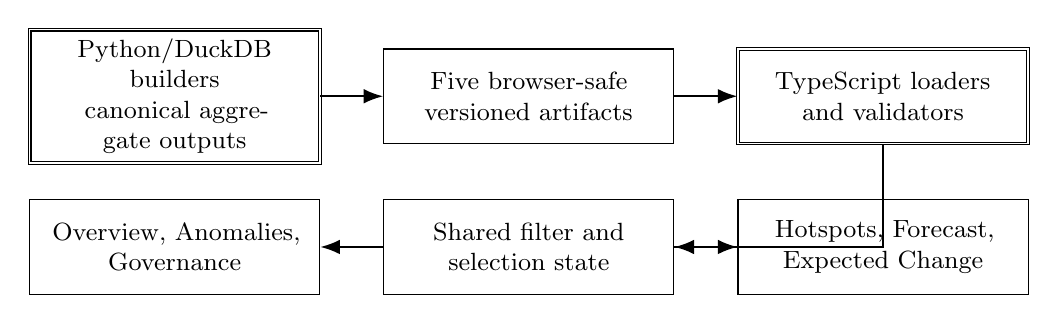
\begin{tikzpicture}[
    node distance=7mm and 8mm,
    block/.style={draw=black,
      minimum height=12mm, text width=3.45cm, align=center,
      font=\small},
    active/.style={block, double},
    arrow/.style={-{Latex[length=2.5mm]}, thick}
  ]
    \node[active] (builders) {Python/DuckDB builders\\canonical aggregate outputs};
    \node[block, right=of builders] (contracts) {Five browser-safe\\versioned artifacts};
    \node[active, right=of contracts] (loaders) {TypeScript loaders\\and validators};
    \node[block, below=of contracts] (state) {Shared filter and\\selection state};
    \node[block, left=of state] (views1) {Overview, Anomalies,\\Governance};
    \node[block, right=of state] (views2) {Hotspots, Forecast,\\Expected Change};
    \draw[arrow] (builders) -- (contracts);
    \draw[arrow] (contracts) -- (loaders);
    \draw[arrow] (loaders) |- (state);
    \draw[arrow] (state) -- (views1);
    \draw[arrow] (state) -- (views2);
  \end{tikzpicture}
  \caption{Dashboard data flow. The browser receives only validated aggregate
  artifacts; raw complaint rows never cross the browser boundary.}
  \label{fig:dashboard-architecture}
\end{figure}

Optional sources remain independent. A missing forecast, hotspot, anomaly, or
spatial artifact is not silently converted into an empty result or numeric zero.
The UI distinguishes a valid zero, an available-but-empty result, a
filter-produced empty state, missing history, an incompatible artifact, and a
network failure.

\section{Spatial reference and map resilience}

Forecast and Expected Change use official \texttt{MultiPolygon} boundaries from
the NYC Department of City Planning / NYC Open Data Police Precincts dataset,
identifier \texttt{y76i-bdw7}, edition 26B. The spatial contract covers all 78
forecast precinct keys exactly once. It does not substitute complaint-derived
hotspot centroids for administrative boundaries.

Raster tiles provide visual context but are not required for analytical access.
If CARTO tiles fail, vector polygons or points, filters, legends, lists, and
detail panels remain available. Geometry is withheld after a declared 120-day
review window unless a new edition is reviewed; forecast list and detail values
remain accessible even when polygons are stale.

\chapter{Analytical Views and Interaction Design}

\section{Overview}

The Overview view combines a shared filter toolbar with metric cards, a weekly
volume series, borough and offense comparisons, law-category totals, and a
priority-signal table. The default complete-week window contains 567,306
reported rows, a recent four-week change of $-12.8\%$, 26 high or critical
hotspots, 645 high or critical anomalies, and a next-week point estimate of
8,168.3. These values are contextual summaries, not operational alerts.

\begin{figure}[htbp]
  \centering
  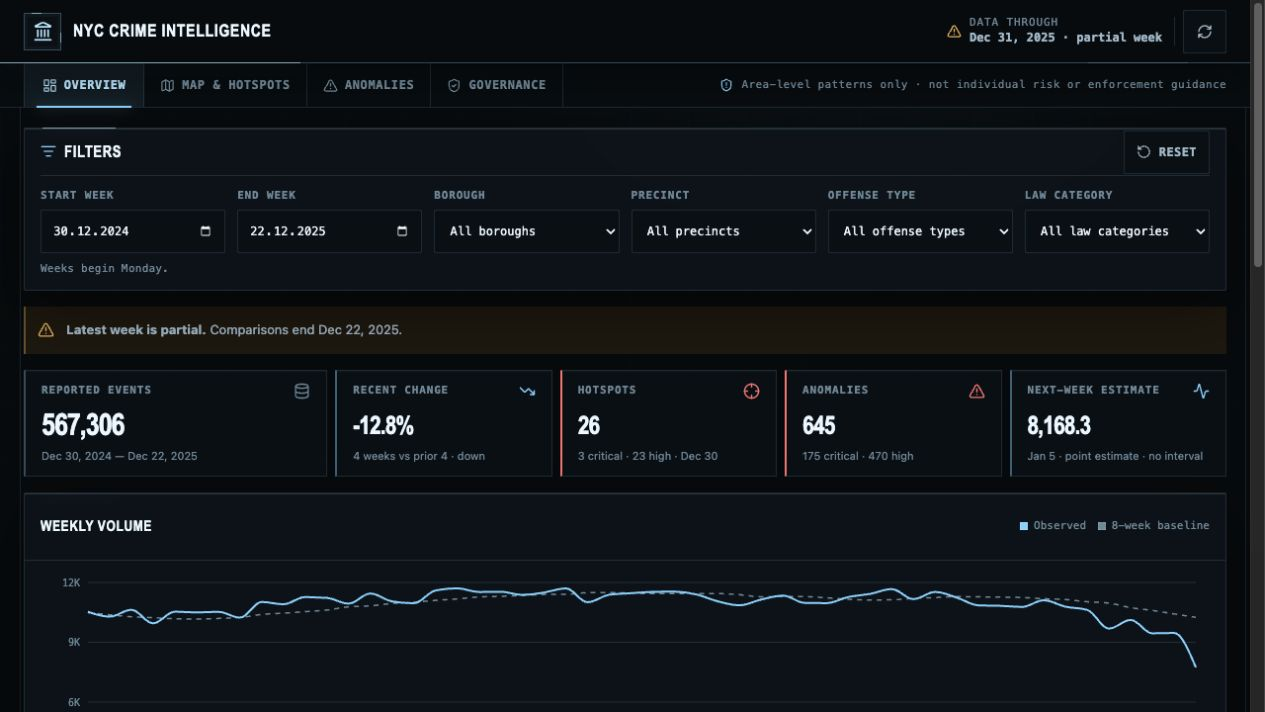
\includegraphics[width=\textwidth]{dashboard-overview.png}
  \caption{Overview interface with shared filters, aggregate metrics, partial-week
  warning, and observed-versus-baseline weekly trend.}
  \label{fig:dashboard-overview}
\end{figure}

Date filters select inclusive Monday-starting buckets. The recent-change card
uses up to four selected complete weeks and compares them with the directly
preceding equal-length window; partial weeks are excluded from this comparison.

\section{Map workspace: Hotspots, Forecast, and Expected Change}

The Map workspace contains three analytical modes under one set of categorical
filters.

\subsection{Hotspots}

Hotspots are a fixed retrospective snapshot dated December 30, 2025. The
method compares a recent 30-day count with a non-overlapping 365-day baseline;
7- and 90-day counts provide recency context. The composite score is:

\begin{equation}
0.35D + 0.25L + 0.20S + 0.15R + 0.05Q,
\end{equation}

where $D$ is density, $L$ baseline lift, $S$ share increase, $R$ recency, and
$Q$ coordinate quality. The reviewed output contains 396 signals: 36 precinct
and 360 grid records, of which 26 are high or critical \cite{hotspotreport}.

\begin{figure}[htbp]
  \centering
  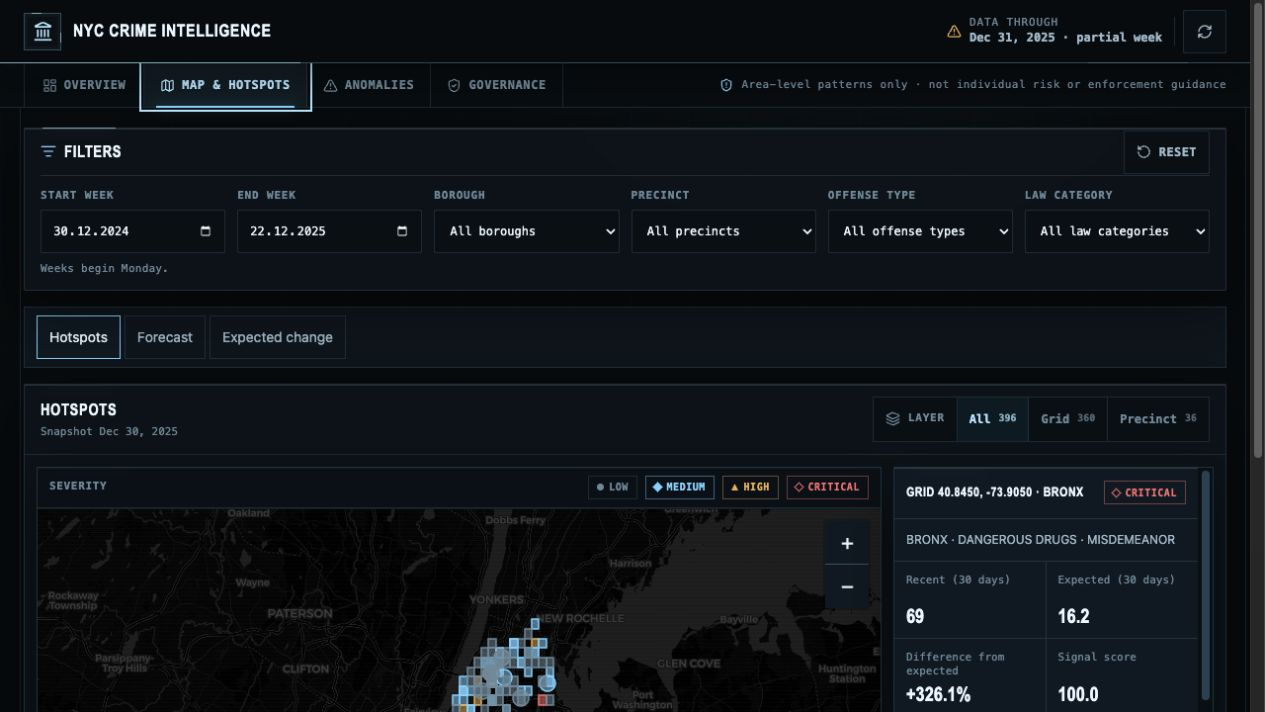
\includegraphics[width=\textwidth]{dashboard-hotspots.png}
  \caption{Hotspot mode with severity legend, aggregate map markers, and a
  synchronized detail panel. A full list/detail path is available below the map.}
  \label{fig:dashboard-hotspots}
\end{figure}

Grid points are 0.01-degree cell centers, and precinct points are aggregate
centroids. Neither is an exact complaint location. The grid is not equal-area,
and hotspot scores do not measure causality, offense seriousness, neighborhood
danger, or action priority.

\subsection{Forecast}

Forecast mode aggregates filtered model rows to one point estimate per precinct
for the fixed week beginning January 5, 2026. Polygons, list entries, and detail
panels share one selection state. Date filters only determine whether this fixed
horizon is compatible with the selected context; they do not create new
forecast dates.

\subsection{Expected Change}

Expected Change displays the forecast minus the prior-only trailing eight-week
arithmetic mean. Baselines are aggregated only when every contributing row has
sufficient history. If any required baseline is unavailable, change is withheld
instead of treating missing history as zero. A valid zero baseline remains zero,
and its percentage change is shown as undefined rather than infinite.

\section{Anomalies}

Anomalies are already-observed weekly aggregates that exceed a prior-only
historical expectation. The detector uses trailing 8- and 13-week means, a
13-week standard deviation, and a 26-week median and median absolute deviation.
When aligned, the expected value can use a leakage-safe model backtest estimate;
otherwise it uses the prior 13-week mean.

The analytical output contains 89,362 flagged rows. The browser projection
retains 10,378 high or critical records, with 645 in the default complete-week
window. Rows expose actual, expected, residual, score, source, and severity.
They are retrospective deviations, not probabilities or forecasts
\cite{anomalyreport}.

\section{Governance}

Governance is filter-independent and reconciles allowlisted metadata from the
same dashboard artifacts. It presents:

\begin{itemize}
  \item source coverage and row populations;
  \item overlapping quality flags and retained \texttt{UNKNOWN} values;
  \item model identity, versions, validation windows, artifact readiness, and
    lifecycle timestamps;
  \item known analytical and product limitations; and
  \item responsible-use and prohibited-use boundaries.
\end{itemize}

The view deliberately separates the source-data horizon, artifact generation
time, and the unavailable independent training-completion time. It does not
manufacture a generic health label or infer facts that the project did not
record.

\chapter{Accessibility, Verification, and Operations}

\section{Accessible and responsive behavior}

The dashboard uses native landmarks, headings, controls, lists, and status
semantics. Map views have a complete list/detail path so an analyst does not
need to operate the map with a pointer. Anomaly and spatial list rows are native
buttons; visible selection, detail content, and polite status messages share a
stable identity.

Severity is communicated through text and shape as well as color. Touch targets
have a 44-pixel minimum, visible focus is preserved, and desktop, tablet, and
mobile layouts avoid page-level horizontal overflow. Reduced-motion preferences
remove or simplify transitions, while structural borders and solid-color
fallbacks preserve content where blur or transparency are unavailable.

Automated tests cover native button activation, focus visibility, and selection
synchronization. The remaining documented task is a final manual repetition of
precinct-list keyboard activation on the intended browser and platform.

\section{Automated verification}

The repository-wide command \texttt{./scripts/verify\_local.sh} checks Python
contracts, documentation and repository hygiene, locked frontend installation,
ESLint, Vitest, TypeScript compilation, the Vite production build, the production
dependency audit, whitespace, and local port hygiene.

The reviewed acceptance pass on July 19, 2026 completed:

\begin{itemize}
  \item 136 Python contract tests;
  \item 214 Vitest tests;
  \item ESLint and the TypeScript/Vite production build;
  \item production dependency audit;
  \item privacy, path, notebook, history, documentation, and whitespace checks;
    and
  \item desktop, tablet, mobile, state, tile-failure, console, and network
    review scenarios.
\end{itemize}

An optional full-data integration mode rebuilds the Overview, Map, Forecast Map,
and compressed cube outputs from ignored local inputs and compares them exactly
with the committed browser-safe artifacts.

\section{Refresh and release workflow}

The analytical dependency order is fixed. A full refresh runs cleaning,
summary construction, baseline forecasting, ML forecasting, hotspots,
anomalies, Overview projection, Map projection, Forecast Map projection, and
spatial-reference projection. The explicit cleaning review date must advance
only with a deliberate source refresh.

Canonical artifacts under \path{data/processed/} and their staged counterparts
under \path{dashboard/public/data/} must remain byte-identical. Browser JSON
must not be hand-edited, source-derived dates must not be replaced with wall
clock time, and paths outside the declared repository root are rejected by the
builders.

\section{Dashboard limitations}

The dashboard improves transparency but cannot eliminate the limitations of its
source and model:

\begin{itemize}
  \item the forecast is fixed and retrospective rather than live;
  \item all forecasts are point estimates without uncertainty intervals;
  \item hotspot thresholds are fixed and grid cells are unequal in area;
  \item precinct geometry depends on a separately reviewed quarterly source;
  \item raster context depends on an external tile provider; and
  \item overall historical errors do not guarantee accuracy for active filters.
\end{itemize}

The interface addresses these limits through explicit dates, partial-week
warnings, model and baseline context, distinct unavailable states, a Governance
view, aggregate-only data contracts, and repeated responsible-use language.

\chapter*{Conclusion}
\addcontentsline{toc}{chapter}{Conclusion}

NYC Crime Intelligence demonstrates a coherent path from a large public source
dataset to an auditable forecasting artifact and a defensive browser interface.
Its strongest design decisions are the deterministic cleaning contract,
prior-only feature construction, time-ordered evaluation, transparent lag
formula, explicit baseline comparison, and strict separation between aggregate
analytics and person-level or operational decision-making.

The lag ensemble produces a measurable but modest error reduction. That result
supports the project's restrained product posture: the model is useful as an
explainable retrospective demonstration, but it does not justify real-time or
high-stakes use. The dashboard carries this conclusion into the interface by
preserving time semantics, exposing limitations, distinguishing unavailable
states from zero, and keeping all complaint-level and demographic information
out of the browser.

Future technical work should prioritize matched-row model comparisons,
prediction intervals and calibration, holiday and reporting-delay features,
drift monitoring, a documented retraining policy, equal-area or better justified
spatial methods, and completion of the final manual accessibility review.

\appendix
\chapter{Reproduction Commands}

\section{Python environment}

\begin{verbatim}
python3.11 -m venv .venv
source .venv/bin/activate
python -m pip install -r requirements.txt
\end{verbatim}

\section{Full analytical rebuild}

\begin{verbatim}
.venv/bin/python src/data/build_clean_dataset.py \
  --as-of-date 2026-07-04
.venv/bin/python src/analytics/build_dashboard_summary.py
.venv/bin/python src/models/build_baseline_forecast.py
.venv/bin/python src/models/build_ml_forecast.py
.venv/bin/python src/analytics/build_hotspots.py
.venv/bin/python src/analytics/build_anomalies.py
.venv/bin/python src/analytics/build_dashboard_overview.py
.venv/bin/python src/analytics/build_dashboard_map.py
.venv/bin/python src/analytics/build_dashboard_forecast_map.py
.venv/bin/python \
  src/analytics/build_dashboard_precinct_spatial_reference.py
\end{verbatim}

\section{Verification and dashboard startup}

\begin{verbatim}
./scripts/verify_local.sh
./scripts/verify_local.sh --full-data
./run.sh
\end{verbatim}

\clearpage
\begin{thebibliography}{99}

\bibitem{rootreadme}
NYC Crime Intelligence Project.
\emph{Repository README}.
\path{README.md}, reviewed July 19, 2026.

\bibitem{finalreport}
NYC Crime Intelligence Project.
\emph{Final Project Report}.
\path{reports/final_project_report.md}, July 19, 2026.

\bibitem{provenance}
NYC Crime Intelligence Project.
\emph{NYPD Complaint Data Historic Provenance Note}.
\path{data/source/nyc_open_data/nypd_complaint_data_historic.md}.

\bibitem{cleaningreport}
NYC Crime Intelligence Project.
\emph{Cleaning and Aggregation Report}.
\path{reports/cleaning_report.md}, July 4, 2026.

\bibitem{qualityreport}
NYC Crime Intelligence Project.
\emph{Data Quality Report}.
\path{reports/data_quality_report.md}.

\bibitem{baselinereport}
NYC Crime Intelligence Project.
\emph{Baseline Forecast Model Report}.
\path{reports/baseline_model_report.md}, July 5, 2026.

\bibitem{baselinemanifest}
NYC Crime Intelligence Project.
\emph{Baseline Forecast Model Manifest, Artifact Version 1}.
\path{models/baseline_forecast/model_manifest.json}.

\bibitem{mlreport}
NYC Crime Intelligence Project.
\emph{ML Forecast Model Report}.
\path{reports/ml_model_report.md}, July 5, 2026.

\bibitem{mlmanifest}
NYC Crime Intelligence Project.
\emph{Weekly Forecast Model Manifest, Model Version 1 and Artifact Version 1}.
\path{models/weekly_forecast/model_manifest.json}.

\bibitem{hotspotreport}
NYC Crime Intelligence Project.
\emph{Hotspot Methodology}.
\path{reports/hotspot_methodology.md}.

\bibitem{anomalyreport}
NYC Crime Intelligence Project.
\emph{Anomaly Methodology}.
\path{reports/anomaly_methodology.md}.

\bibitem{dashboardreadme}
NYC Crime Intelligence Project.
\emph{Dashboard Architecture and Operations Guide}.
\path{dashboard/README.md}, reviewed July 19, 2026.

\bibitem{nycopendata}
City of New York.
\emph{NYPD Complaint Data Historic (qgea-i56i)}.
\url{https://data.cityofnewyork.us/Public-Safety/NYPD-Complaint-Data-Historic/qgea-i56i}.

\end{thebibliography}

\end{document}
